\addsection{All Map Locations}{\images/ballistics.png}
\begin{wrapfigure}{R}{0.5\textwidth}
    \begin{center}
    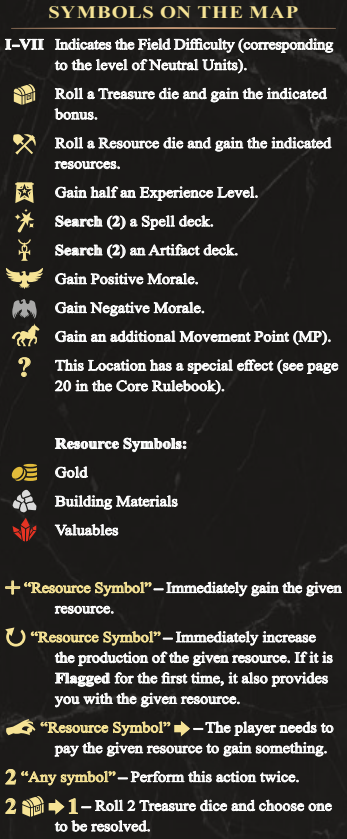
\includegraphics[width=0.48\textwidth]{\images/symbols.png}
    \end{center}
\end{wrapfigure}
\hypertarget{All}{This} section describes the function of every single field in the game.
The vast majority of fields have useful iconography that clearly communicates the field's effect.
On the right is a screenshot of the back of the rule book that explains these.
If a field has any combination of these icons and is not described in detail later, then that field is either \textbf{visitable} or \textbf{flaggable} and its only effect is indicated by these icons.\par
Revisitable fields do not have an icon that indicates them to be such.
For this reason all revisitable fields are pictured and described individually.
The 
\includegraphics[scale=0.75]{\images/revisitable.png} symbol is on almost all flaggable fields, with the major exception of settlements.
Rules for flagging mines, settlements and towns are on the next page followed by descriptions of revisitable and unique fields marked with a question mark.\par
Random towns are explained above.

\clearpage
\subsection*{Towns, mines and settlements}
\textbf{Towns} are always located in the center of a starting tile.
Flagging an enemy town prevents their secondary heroes from spawning there and main heroes from moving there if defeated.
Flagging a town can cause \hyperlink{End}{player elimination}, and scenarios typically have special rewards for flagging them.
Flagging a town also gives you a faction cube from its original owner.
Otherwise, flagging a town does not affect its original owner in any way.
They do not lose access to their town board or its functions.
You also do not gain access to their town board or faction units, unlike in the video game.
You can \hyperlink{Town}{pay gold} to defend towns with units.\\
\begin{figure}[h]
\centering
\shadowimage[width=0.5\linewidth]{\images/core_towns.jpg}
\caption{\textit{Towns from the core game.}}
\end{figure}

\textbf{Mines} are flaggable fields which increase a specific resource's income when flagged.
If you are the first one to flag a mine, it also immediately provides you with its income.

\begin{figure}[h]
\centering
\shadowimage[width=0.25\linewidth]{\images/mine_example.png}\\
\caption{\textit{A mine that produces valuables, guarded by level 3 neutrals.
  The first player to flag this field would immediately gain one valuable in addition to increasing their valuables income.
  All mines have the 
\includegraphics[scale=0.5]{\images/revisitable.png} symbol.}}
\end{figure}

\textbf{Settlements} function similarly to both towns and mines.
They act as a spawn point for secondary heroes, and as a place for main heroes to move to when defeated.
You may also \hyperlink{Town}{pay gold} to defend settlements with units.
When you flag a settlement, you choose whether to increase your \textbf{gold}, \textbf{building materials} or \textbf{valuables} income by one space.
As with mines, if you are the first player to flag a settlement, you immediately gain resources equal to that increase in production.
Mark the settlement with an appropriate resource token to show which resource it produces.
When you flag an enemy settlement you may switch which resource it produces.\par
Additionally, \textbf{instead of increasing resource production}, you may choose to \textbf{reinforce} one of your bronze or silver units immediately for half the normal cost, rounded up.
If you were the first player to flag the settlement, reinforce that unit for free instead.
Do not place any resource tokens on the settlement if you choose to reinforce.
\begin{figure}[h]
\centering
\shadowimage[width=.3\textwidth]{\images/castle_settlement.jpg}\hfill%
\shadowimage[width=.3\textwidth]{\images/dungeon_settlement.jpg}\hfill%
\shadowimage[width=.3\textwidth]{\images/necropolis_settlement.jpg}\\
\vspace{4pt}
\shadowimage[width=.3\textwidth]{\images/rampart_settlement.jpg}\hfill%
\shadowimage[width=.3\textwidth]{\images/fortress_settlement.jpg}\hfill%
\shadowimage[width=.3\textwidth]{\images/inferno_settlement.jpg}\\
\vspace{4pt}
\shadowimage[width=.3\textwidth]{\images/tower_settlement.jpg}\\%
\vspace{4pt}
\textit{All possible settlements.
  Each is styled after a different faction.
  They all work identically.}
\end{figure}
\bigbreak

\subsection*{Revisitable fields}
\begin{figure}[h]
  \centering
  \captionsetup{width=.5\linewidth}
  \textbf{Stables}\par\medskip
  \shadowimage[width=0.5\linewidth]{\images/stables.jpg}
  \caption{Category: \textbf{Revisitable}\\Gain 1 additional MP.}
  \bigbreak
  \textit{
    This movement point lasts for only one turn.
    The same is true for all other effects which grant MP.
    Essentially, it's "free" to move onto this field.
  }
\end{figure}

\begin{figure}
  \begin{minipage}[t]{0.48\textwidth}
    \centering
    \textbf{Library}\par
    \shadowimage[width=\textwidth]{\images/library.jpg}
    \caption{Category: \textbf{Revisitable}\\You can
      \includesvg[height=10px]{\svgs/pay_v2.svg}
      3 \includesvg[height=10px]{\svgs/gold.svg}
      to Remove 1 Statistic card from   your hand or discard pile and replace it with any other Statistic card.
      You can do it twice per visit.}
  \end{minipage}\hfill
  \begin{minipage}[t]{0.48\textwidth}
    \centering
    \captionsetup{singlelinecheck=off}
    \textbf{Black Market}\\
    \shadowimage[width=\textwidth]{\images/black_market.jpg}
    \caption[black market]{Category: \textbf{Revisitable}\\Look at the top 4 cards from the Artifact discard pile.
      You can buy one of them for:
      \begin{itemize}
        \item [5] \includesvg[height=10px]{\svgs/gold.svg} if it is a \textbf{Minor} Artifact
        \item [7] \includesvg[height=10px]{\svgs/gold.svg} if it is a \textbf{Major} Artifact
        \item [10] \includesvg[height=10px]{\svgs/gold.svg} if it is a \textbf{Relic} Artifact
      \end{itemize}
      }
  \end{minipage}
\end{figure}

\begin{figure}
  \begin{minipage}[t]{0.48\textwidth}
    \centering
    \textbf{Sanctuary}\\
    \shadowimage[width=\textwidth]{\images/sanctuary.jpg}
    \caption{Category: \textbf{Revisitable}\\
      Heroes on this field cannot be attacked by other Heroes.
      If a field is occupied by a Hero, other Heroes can move through but cannot stop here.}
  \end{minipage}\hfill
  \begin{minipage}[t]{0.48\textwidth}
    \centering
    \textbf{Tavern}\par
    \shadowimage[width=\textwidth]{\images/tavern.jpg}
    \caption{Category: \textbf{Revisitable}\\You can \includesvg[height=10px]{\svgs/pay_v2.svg}
    7 \includesvg[height=10px]{\svgs/gold.svg}
    on this field to gain a Secondary Hero and choose one enemy player to discard 1 random card from their hand.}
  \end{minipage}
\end{figure}

\begin{figure}
  \begin{minipage}[t]{0.48\textwidth}
    \centering
    \hypertarget{Trading Post}{\textbf{Trading Post}}\\
    \shadowimage[width=\textwidth]{\images/trading_post.jpg}
    \caption{Category: \textbf{Revisitable}\\
      Exchange resources or Remove a card.
      See \protect\hyperlink{Trading}{trading}.}
  \end{minipage}
\end{figure}

\clearpage

\subsection*{Other fields}
The effects of these fields are only indicated by a question mark on their tiles.\par
\bigbreak
\begin{figure}[h]
  \begin{minipage}[t]{0.48\textwidth}
    \centering
    \textbf{Tree Of Knowledge}\\
    \shadowimage[width=\linewidth]{\images/tree.jpg}
    \caption{Category: \textbf{Visitable}\\You may
      \includesvg[height=10px]{\svgs/pay_v2.svg}
       3 \includesvg[height=10px]{\svgs/valuablegreater.svg} or
       10 \includesvg[height=10px]{\svgs/gold.svg} to gain
       2 \includesvg[height=10px]{\svgs/exp.svg}.}
  \end{minipage}\hfill
  \begin{minipage}[t]{0.48\textwidth}
    \centering
    \textbf{Redwood Observatory}\\
    \shadowimage[width=\linewidth]{\images/observatory.jpg}
    \caption{Category: \textbf{Visitable}\\Discover a tile adjacent to this one.}
  \end{minipage}
\end{figure}

\begin{figure}[h]
  \begin{minipage}[t]{0.48\textwidth}
    \centering
    \textbf{Grail}\\
    \shadowimage[width=\linewidth]{\images/grail.jpg}
    \caption{Category: \textbf{Visitable}\\
      Gain a Grail token.}
  \end{minipage}\hfill
  \begin{minipage}[t]{0.48\textwidth}
    \centering
    \textbf{Dragon Utopia}\\
    \shadowimage[width=\linewidth]{\images/dragon_utopia.jpg}
    \caption{Category: \textbf{Flaggable}\\Effects depend on scenario.}
  \end{minipage}
\end{figure}

\begin{figure}[h]
  \begin{minipage}[t]{0.48\textwidth}
    \centering
    \textbf{Market Of Time}\\
    \shadowimage[width=\linewidth]{\images/market_of_time.jpg}
    \caption{Category: \textbf{Visitable}\\ Remove one card from your hand.
Then \textbf{Search (2)} Ability, Spell, or Artifact deck.}
  \end{minipage}\hfill
  \begin{minipage}[t]{0.48\textwidth}
    \centering
    \textbf{University}\\
    \shadowimage[width=\linewidth]{\images/university.jpg}
    \caption{Category: \textbf{Visitable}\\
      \includesvg[height=10px]{\svgs/pay_v2.svg} 6 \includesvg[height=10px]{\svgs/gold.svg} to \textbf{Search (4)} the Ability discard pile.}
  \end{minipage}
\end{figure}

\begin{figure}[h]
  \begin{minipage}[t]{0.48\textwidth}
    \centering
    \textbf{Magic Spring}\\
    \shadowimage[width=\linewidth]{\images/magic_spring.jpg}
    \caption{Category: \textbf{Visitable}\\
      You may look at the top 3 cards of your discard pile and take 1 of them back to your hand.
      Return the remaining cards on top of your discard pile in any order.}
  \end{minipage}\hfill
  \begin{minipage}[t]{0.48\textwidth}
    \centering
    \textbf{Witch Hut}\\
    \shadowimage[width=\linewidth]{\images/witch_hut.jpg}
    \caption{Category: \textbf{Visitable}\\
      You may either Remove an Ability card from your hand or look at the top card of the Ability deck and put that card into your hand or into the Ability deck discard pile.}
  \end{minipage}
\end{figure}

\begin{figure}[h]
  \begin{minipage}[t]{0.48\textwidth}
    \centering
    \textbf{Obelisk}\\
    \shadowimage[width=\linewidth]{\images/obelisk.jpg}
    \caption{Category: \textbf{Flaggable}\\
      An Obelisk's effects can vary depending on the scenario.
      When you visit it, the enemy faction cubes are not removed, meaning that there may be multiple cubes on the field.
      Once visited by a faction, the Obelisk counts as an empty field for that faction, just like a visitable field would.}
  \end{minipage}\hfill
  \begin{minipage}[t]{0.48\textwidth}
    \centering
    \textbf{Star Axis}\\
    \shadowimage[width=\linewidth]{\images/star_axis.jpg}
    \caption{Category: \textbf{Flaggable}\\
      You can Remove one of your Statistic cards from your hand and replace it with an Empowered one of the same type.
      When you visit a Star Axis, the enemy faction cubes are not removed, meaning that there may be multiple cubes on the field.
      Once visited by a faction, the Star Axis counts as an empty field for that faction, just like a visitable field would.
    }
  \end{minipage}
\end{figure}

\begin{figure}
  \begin{minipage}[t]{0.48\textwidth}
    \centering
    \textbf{Hill Fort}\\
    \shadowimage[width=\linewidth]{\images/hill_fort.jpg}
    \caption{Category: \textbf{Visitable}\\
      You can immediately Reinforce one of your \includesvg[height=10px]{\svgs/bronze.svg} or \includesvg[height=10px]{\svgs/silver.svg} units.
      The Reinforcement cost is reduced by 3 \includesvg[height=10px]{\svgs/gold.svg} to a minimum of 0.}
  \end{minipage}\hfill
  \begin{minipage}[t]{0.48\textwidth}
    \centering
    \textbf{Prison}\\
    \shadowimage[width=\linewidth]{\images/prison.jpg}
    \caption{Category: \textbf{Visitable}\\
      You gain a Secondary Hero.
      Place their model on this field.
      If you already have a Secondary Hero, gain 3 \includesvg[height=10px]{\svgs/gold.svg}.}
  \end{minipage}
\end{figure}

\begin{figure}
  \captionsetup{singlelinecheck=off, width=.5\linewidth}
  \centering
  \textbf{Scholar}\par\medskip
  \shadowimage[width=0.5\linewidth]{\images/scholar.jpg}
  \caption[scholar they]{Category: \textbf{Visitable}\\
    Roll 1 Attack die.
    Depending on the result, do the following:
    \begin{itemize}
      \item[ \textbf{+1}] - Draw 1 chosen Statistic card or Remove one of the Statistic cards from hand.
      \item[\textbf{0}] - Draw 2 Ability cards, take one of them and discard the other.
      \item[\textbf{-1}] - Draw 2 Spell cards, take one of them and discard the other.
      \end{itemize}
     }
     \bigbreak
     \textit{
        The scholar's "drawing" of statistic cards refers to the piles of unused basic statistics cards.
        Removing a statistic card should work with empowered statistics too.
        Their other abilities are basically searching without the option of taking a discarded card.
      }
\end{figure}
